\documentclass[10pt]{article}
\usepackage{amsmath}
\usepackage{amsfonts}
\usepackage{amssymb}

\usepackage{graphicx}

\author{Sawaiz Syed}
\title{Design for networked radiation sensor for production}

\begin{document}
\maketitle

\section{Introduction}
Cosmic ray radiation from outside our solar system are powerful gamma rays that disperse 
after hitting out atmosphere. As we move closer to the edge of our atmosphere, their 
energy increases \cite{Nave}. About 90\% of cosmic rays are protons, and 9\% 
are alpha particles \cite{Nave}. These very high energy particles (called 
primaries)Strike the upper layer of the atmosphere and transfer their energy into 
particles classified as secondaries. The secondary rays consist of pions (that decay 
to muons, neutrinos, and gamma rays) and electrons and positrons \cite{Mewaldt1996}. The 
Figure~\ref{fig:atmosphericCascade} shows the how the atmospheric cascade reduces the energy of 
the primary particle into multiple weaker secondaries, if the energy of the primary 
is above 500MeV, the secondaries will still reach earth's surface before dissipation 
\cite{Bieber2000}. 

\begin{figure}[h]
	\centering
    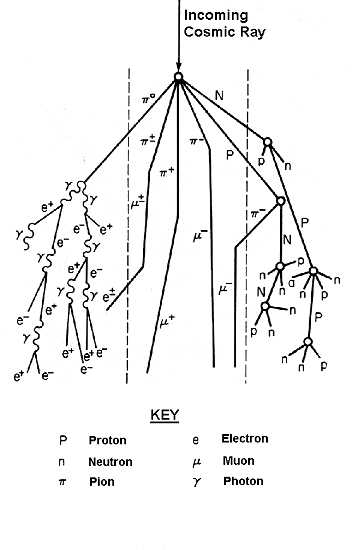
\includegraphics[width=0.5\textwidth]{atmosphericCascade.png}
    \caption{Atmospheric cascade.}
    \label{fig:atmosphericCascade}
\end{figure}

The average energy of primary particles is 1GeV (corresponding to .87C) 
although TeV occurrences have been measured.\cite{Nave}. While at sea level the 
radiation caused by the particles is low with an intensity of $100 \frac{particles}{m^2s}$ 
\cite{Mewaldt1996}, it can still cause memory electronic errors, and health effects to 
aviation \cite{Friedberg2000} and space personnel.

\subsection{Previous Research}
The sensors currently available for radiation detection are expensive, devices made 
once with limited documentation to how they work, and are used. They provide a very 
small set of data, and at only a single location, generally inside a climate controlled 
lab. The devices are designed without the consideration of making more devices, and 
creating additional devices adds greatly to both the cost and time. Previously data 
has been collected and used, but in very limited amounts. The data collected has been 
from distant locations such as the radiation sensor on campus, while the weather 
readings are measured from Peachtree City Observation Station \cite{Dayananda2013}, 
approximately thirty miles away this provides general readings but the weather variance 
can be so great between those locations that precise coloration is difficult to 
accomplish. The newer results use a weather station atop the building, but the sensors 
are physically too close that all the data from the detectors would not give 
information on the larger scale.

\subsection{Infrastructure}
With city infrastructure getting denser and complex, the threat of dirty bombs and 
danger from nuclear power facilities pose a risk in tightly packed urban areas. 
Detecting radiation on such a scale is difficult, expensive, and is difficult to 
justify the cost when the funds can be allocated to other infrastructure. Small 
inexpensive mountable mesh of sensors can provide real time location based
radiation readings and sensors mounted on public transit and government vehicles would also 
provide geolocation data for trackable readings. These could give information critical 
to the current security for anti terrorism, public safety, and long term data that provides information
on how average radiation readings fluctuate.

\subsection{Workplace}
In locations where retroactively hazardous materials could be handled this information can
be helpful to mitigate problems caused by human error. An example scenario could be a worker 
dealing with radioactive materials, leaving the room without placing the sample back into storage.
The system could also warn the personnel overseeing a nuclear power plant of any leaks of contamination
due to the larger amount of area the sensors would cover at the same cost as currently used sensors.

\subsection{Current Options}
The options for the collection of current data has been very sparse. Small hand held sensors can
provide data that would either have to be manually logged, along with the location and hence is 
highly impractical. Other options include addons to weather stations, and computers with many 
sensors connected via USB, and modular sensor systems. But the major problem with 
all these options is the physical size and high power consumption that limits the locations and 
areas the devices can be placed. Most devices have a volume of ten to one hundred times the 
volume of the sensing apparatus, and a power consumption on the order of ten to hundreds of 
milliamps, that is too high for long term data logging.

\subsection{Requirements}
An ideal sensor setup would consist of a physically small sensor with very low power consumption. 
Multiple transmitters with little computing all sending to a single internet connected receiver 
with error checking. It should be physically strong, easily mountable, and weather proof. Finally
the unit should be designed for manufacturing to make the cost per unit as low as possible. The 
device should have good code and hardware documentation for further research and for others to use 
it as a platform for making other sensors.

\pagebreak
\bibliographystyle{plain}
\bibliography{RadiationSensor}

\end{document}